\documentclass[tikz,border=10pt]{standalone}

\usepackage{ctex}
\usepackage{tikz}
\usepackage{fontspec}

\usetikzlibrary{
    shapes.geometric,
    arrows.meta,
    positioning
}


% Code font
% \setmonofont{DejaVu Sans Mono}
% \setmainfont{TeX Gyre Pagella}
\setmainfont{Segoe Print}


\begin{document}


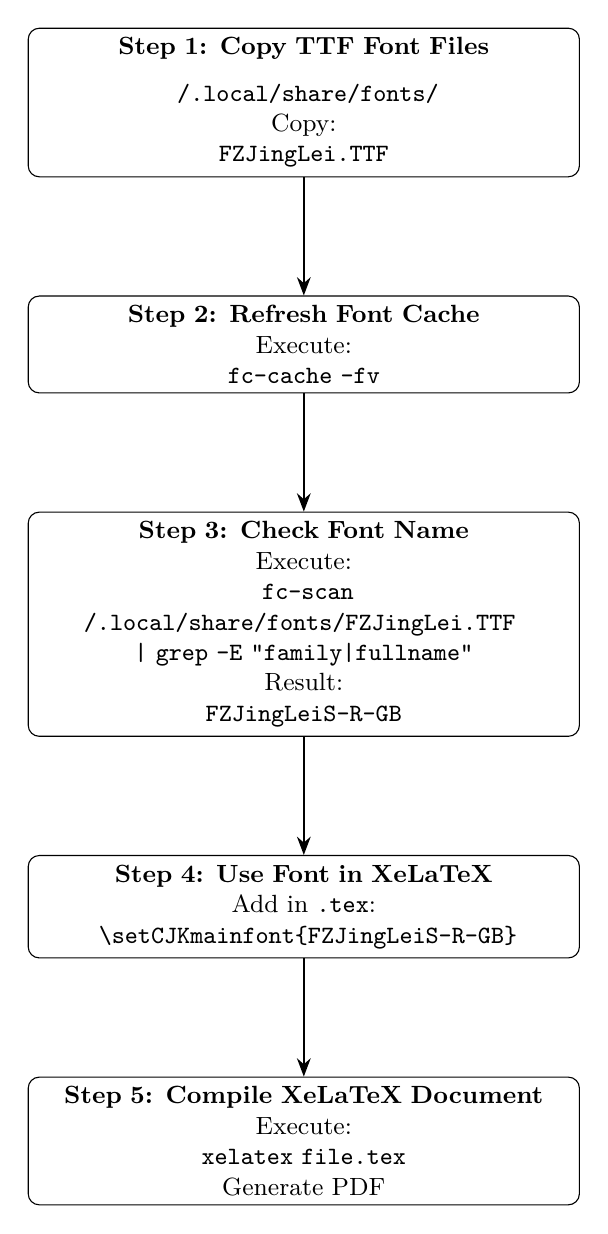
\begin{tikzpicture}[
    node distance=1.5cm,
    every node/.style={
        align=center,
        font=\small
    },
    process/.style={
        rectangle,
        rounded corners,
        draw,
        minimum width=7cm,
        minimum height=1.2cm,
        text width=6.5cm
    },
    arrow/.style={
        -{Stealth},
        thick
    }
]


% Step 1

\node[process] (step1)
{
    \textbf{Step 1: Copy TTF Font Files}

    \vspace{0.2cm}

    \texttt{
    ~/.local/share/fonts/
    }

    Copy:

    \texttt{FZJingLei.TTF}
};


% Step 2

\node[process, below=of step1] (step2)
{
    \textbf{Step 2: Refresh Font Cache}

    Execute:

    \texttt{fc-cache -fv}
};



% Step 3

\node[process, below=of step2] (step3)
{
    \textbf{Step 3: Check Font Name}

    Execute:

    \texttt{
    fc-scan ~/.local/share/fonts/FZJingLei.TTF
    }

    \texttt{
    | grep -E "family|fullname"
    }

    Result:

    \texttt{FZJingLeiS-R-GB}
};



% Step 4

\node[process, below=of step3] (step4)
{
    \textbf{Step 4: Use Font in XeLaTeX}

    Add in \texttt{.tex}:

    \texttt{
    \textbackslash setCJKmainfont\{FZJingLeiS-R-GB\}
    }
};



% Step 5

\node[process, below=of step4] (step5)
{
    \textbf{Step 5: Compile XeLaTeX Document}

    Execute:

    \texttt{
    xelatex file.tex
    }

    Generate PDF
};



% arrows

\draw[arrow] (step1) -- (step2);
\draw[arrow] (step2) -- (step3);
\draw[arrow] (step3) -- (step4);
\draw[arrow] (step4) -- (step5);



\end{tikzpicture}


\end{document}
